add additional test, have to be cracked as well, first attacker has to realize them and find them

applied when programming

Environment and Integrity Checks, wenn die umgebung falsch ist, kann die app verändert werden. deswegen von vornherein ausschließen, dass die bedingungen dafür gegeben sind.
\cite{munteanLicense}

mechanisms should work for amazon/lvl/samsung --see- beweis! (amazon die signature den die seite vorgibt?)

force close im falle von falschem outcome, entspricht nicht android qualität
\url{http://developer.android.com/distribute/essentials/quality/core.html} aber so wird es dem user klarer dass seine application gecracked ist. harmlosere variante dialog anzeigen oder element nicht laden.

es gibt verschieden punkte um die integrity der application sicherzustellen. dies beinhaltet die umgebung debugg oder rootzugriff, die suche nach feindliche installierte applicationen oder checks nach der rechtmäßigen installation und rechtmäßigen code.

also works for samsung and amazon

%
in order to remove/disable lvl they have to modify the code
unless done precisely can be detected by code
\cite{developersSecuring}
%


automatischen angriff aushebenln indem andere unbekannte tests die erst entdeckt werden müssen

\begin{figure}[h]
    \centering
    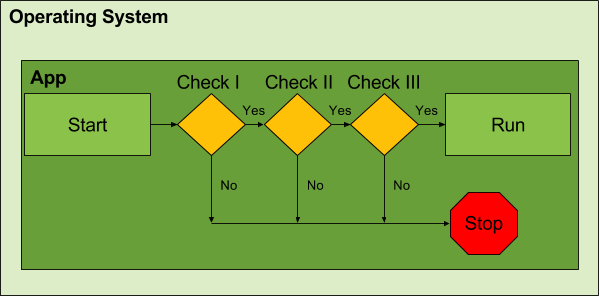
\includegraphics[width=0.8\textwidth]{data/verificationNowAdditional.png}
    \caption{Introduction of additional tests to check environment and integrity of the application}
    \label{fig:verificationNowAdditional}
\end{figure}


%eval
all tampering counter measurements have kind of the same pattern, boolean check, simple method == simple fix, can be nulled easily when code is known, just as easy to crack as LVL when you know the code, but attackr has to invest some time to understand code and to build counter measurement, in addition with Section~\ref{subsection:counter-improve-obfuscation} this can get annoying, evtl create native versions because harder to crack
even though it is simple it adds a little bit extra work to attack and when cobined this grows exponential

but be careful because
annoy people who want to use root
annoy people who bought the app but have luckypatcher/root as well

his does not stop luckypatcher in anyway but it stops the app from working in case the environment is not suitable

but simple method == simple fix
just as easy to crack as LVL when you know the code, can be included in custom patch in luckypatcher after analysing the code and unearthing the fitting patterns to crack
mechanism can be strengthened by creating native versions since it is not as easy to decompile and analyze as dex

but have to be careful since
annoy people who want to use root
annoy people who bought the app but have luckypatcher/root as well

extra arbeit für attacker denn er muss die muster auch finden

!!!signature problem  mit maps überprüfen!!!
